\section{Analisis Hasil Pengujian}

\subsection{Siklus Penjualan Tiket}

Kedua skenario pengujian ini memiliki siklus/fase pola permintaan yang berbeda. Contoh pada skenario beban berkelanjutan diambil dari pengujian f1t2, sedangkan contoh pada skenario perebutan tiket diambil dari pengujian f1t4. Siklus ini juga terjadi pada skenario serupa ketika proses penjualan berjalan dengan lancar.

\subsubsection{Skenario Beban Berkelanjutan}

Pada skenario ini, sistem memiliki ketersediaan tiket yang banyak sehingga penjualan tiket yang berhasil berjalan cukup lama. Pola ini ditunjukkan pada Gambar \ref{fig:pattern-stress-traffic}. Perhatikan bagaimana kurva biru (POST /orders) tetap stabil lalu menurun saat tiket habis, sementara kurva ungu (GET /events/availability/:ticketSaleId) melonjak tajam setelahnya. Ini menandakan fase di mana pengguna beralih dari aktif memesan menjadi hanya memeriksa sisa ketersediaan.

\begin{figure}[H]
    \centering
    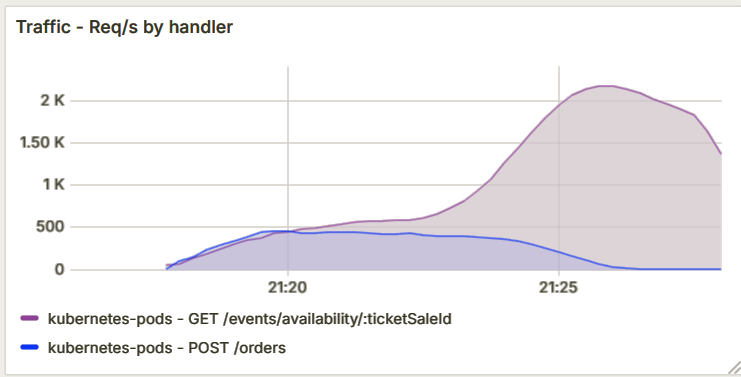
\includegraphics[width=1\textwidth]{resources/chapter-4/pattern-stress-traffic.png}
    \caption{Pola Permintaan pada Beban Berkelanjutan}
    \label{fig:pattern-stress-traffic}
\end{figure}

Status respons pemesanan tiket menunjukkan bahwa terjadi konflik (kode 409) selama pemrosesan pesanan sebanyak 10-12\% dari pemesanan sukses (kode respons 200). Hal ini ditunjukkan pada Gambar \ref{fig:pattern-stress-order}. Pada gambar tersebut, garis merah (kode respons 200) berada pada angka 400 dan garis hijau (kode respons 409) secara rata-rata berada pada angka 50.

\begin{figure}[H]
    \centering
    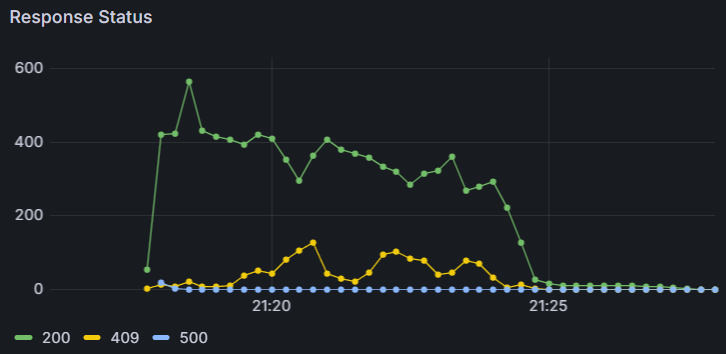
\includegraphics[width=1\textwidth]{resources/chapter-4/pattern-stress-order.png}
    \caption{Status Respons pada Beban Berkelanjutan}
    \label{fig:pattern-stress-order}
\end{figure}

\subsubsection{Skenario Perebutan Tiket}

Pada skenario ini, jumlah permintaan ketersediaan jauh lebih banyak dibandingkan permintaan pemesanan tiket. Hal ini wajar karena terdapat lebih banyak peminat dibandingkan dengan tiket yang tersedia. Berdasarkan Gambar \ref{fig:pattern-sim-traffic}, tiket habis terjual dalam kurang lebih 2,5 menit penjualan. Sistem mulai melayani permintaan pemesanan 2,5 menit sejak pengawasan dimulai dan permintaan pemesanan menjadi nol pada waktu yang ditandai dengan garis hijau (5 menit sejak pengawasan).

\begin{figure}[H]
    \centering
    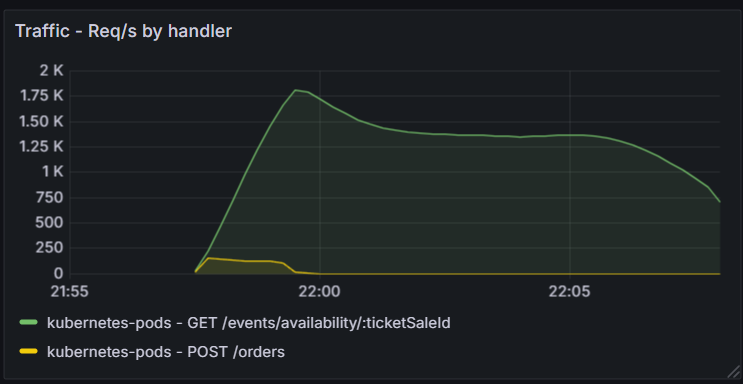
\includegraphics[width=1\textwidth]{resources/chapter-4/pattern-sim-traffic.png}
    \caption{Pola Permintaan pada Perebutan Tiket}
    \label{fig:pattern-sim-traffic}
\end{figure}

Status respons pemesanan tiket menunjukkan bahwa terjadi konflik (kode 409) yang cukup banyak bahkan sejak proses penjualan dimulai. Puncak perebutan terjadi di awal sebagiamana ditunjukkan pada Gambar \ref{fig:pattern-sim-order}. Puncak tertinggi kode respons 409 adalah 400 sedangkan kode respons 200 adalah 250. Pada saat itu, terdapat lebih banyak pesanan yang ditolak dibandingkan dengan pesanan yang berhasil. Pengguna yang baru masuk setelahnya pada akhirnya akan gagal memperoleh tiket, sebagaimana ditunjukkan dengan tidak adanya pesanan yang berhasil setelah penanganan pesanan berjalan beberapa waktu.

\begin{figure}[H]
    \centering
    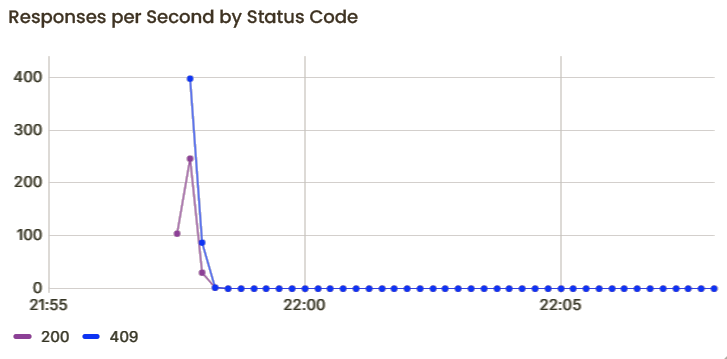
\includegraphics[width=1\textwidth]{resources/chapter-4/pattern-sim-order.png}
    \caption{Status Respons Pemesanan pada Perebutan Tiket}
    \label{fig:pattern-sim-order}
\end{figure}


\subsection{Kinerja Selama Pengujian}

Gambaran kinerja setiap varian basis data ditunjukkan pada Tabel \ref{table:kinerja-pemrosesan-pesanan}. Secara garis besar, varian PostgreSQL mampu menangani beban yang diberikan dengan sangat baik. Varian CitusData masih memiliki kinerja yang baik, meski memiliki latensi yang lebih tinggi dibandingkan dengan PostgreSQL. YugabyteDB mengalami lebih banyak kegagalan dan kinerja yang buruk sehingga tidak dapat menyelesaikan proses penjualan dengan baik. Sampel pengujian yang dipilih pada adalah skenario stress-2 tanpa pengendalian aliran. Skenario ini merupakan skenario pengujian dengan kinerja YugabyteDB yang dapat diterima dan mampu menyelesaikan proses penjualan. Dengan beban yang lebih tinggi, YugabyteDB mengalami banyak kegagalan.

\begin{table}[H]
    \centering
    \caption{Gambaran Kinerja Permosesan Pesanan}
    \label{table:kinerja-pemrosesan-pesanan}
    \begin{tabular}{|l|l|l|l|}
        \hline
        \textbf{Metrik}              & \textbf{PostgreSQL} & \textbf{CitusData} & \textbf{YugabyteDB} \\
        \hline
        \textit{Throughput} Maksimum & 466 rps             & 410 rps            & 216 rps             \\
        \hline
        Penggunaan CPU (Puncak)      & 8 vCPU              & 10 vCPU            & 19 vCPU             \\
        \hline
        Penggunaan Memori (Puncak)   & 3.4 GB              & 5 GB               & 36 GB               \\
        \hline
        Latensi Pemrosesan (P50)     & 192-382 ms          & 496-650 ms         & 854-10000 ms        \\
        \hline
    \end{tabular}
\end{table}

Latensi dan \textit{throughput} pemrosesan diukur dari sisi Ticket Server, bukan dari level basis data. Latensi pemrosesan yang diambil merupakan latensi terbaik saat beban sudah cukup tinggi dan laju pemrosesan mulai stabil. Penggunaan CPU dan penggunaan memori merupakan agregat puncak jumlah penggunaan sumber daya setiap instans basis data yang berkaitan. Apabila terdapat dua nilai maksimal \textit{throughput} yang mendekati, nilai yang dipilih adalah nilai yang memiliki rasio sukses (kode respons 200) paling tinggi.

Berdasarkan Tabel \ref{table:kinerja-pemrosesan-pesanan}, PostgreSQL unggul dari segala aspek, mulai dari laju pemrosesan, penggunaan sumber daya, serta latensi. CitusData memiliki laju pemrosesan yang mendekati PostgreSQL dengan latensi 2x lebih lambat dan penggunaan sumber daya yang sedikit lebih tinggi. Di sisi lain, YugabyteDB memiliki laju pemrosesan kurang dari setengah PostgreSQL dengan latensi setidaknya 4x lebih lambat, penggunaan CPU 2.4x lebih banyak, dan penggunaan memori 10x lebih banyak.

\subsection{Kinerja Basis Data Terdistribusi}

Sebagaimana digambarkan pada Tabel \ref{table:kinerja-pemrosesan-pesanan}, kinerja PostgreSQL lebih baik dibandingkan CitusData dan YugabyteDB. Berikut adalah penelusuran lebih mendalam untuk kinerja setiap basis data, terutama pada skenario lain.

\subsubsection{Rata-Rata Waktu Eksekusi Kueri}

Tabel \ref{table:latensi-kueri} menunjukkan data rata-rata waktu eksekusi kueri yang diambil dari tabel pg\_stat\_statements sesaat setelah pengujian dilaksanakan. Data PostgreSQL diambil dari pengujian f1t2, CitusData diambil dari pengujian f2t3, dan YugabyteDB diambil dari f3t1. Beban antara PostgreSQL dan CitusData sama karena pengujian dijalankan pada skenario stress-0, sedangkan beban pada YugabyteDB lebih ringan karena dijalankan pada skenario stress-2. Data PostgreSQL merupakan gabungan antara statistik pada instans \textit{primary} dan replika. Data mentah merupakan data 10 kueri dengan total eksekusi paling banyak. Kueri yang kosong berarti total eksekusinya tidak cukup signifikan, sehingga dapat diasumsikan latensinya cukup rendah untuk diabaikan dibandingkan dengan yang lain.

\begin{table}[H]
    \centering
    \caption{Latensi Eksekusi Kueri pada Basis Data dalam Milisekon}
    \label{table:latensi-kueri}
    \begin{tabular}{|l|l|l|l|}
        \hline
        \textbf{Kueri}        & \textbf{PostgreSQL} & \textbf{CitusData} & \textbf{YugabyteDB} \\
        \hline
        LockFreeStandingSeats & 8.5                 & 9.8                & 1855                \\
        \hline
        LockNumberedSeats     & -                   & 8.25               & 43                  \\
        \hline
        InsertOrder           & 0.2                 & 4.4                & 77                  \\
        \hline
        UpdateOrder           & -                   & 3.9                & 33                  \\
        \hline
        InsertOrderItem       & 0.24                & -                  & 40                  \\
        \hline
        InsertIssuedTiket     & 0.28                & -                  & 74                  \\
        \hline
        InsertInvoice         & 0.12                & 4.16               & 31                  \\
        \hline
        UpdateInvoice         & 0.12                & 7.7                & -                   \\
        \hline
        UpdateSeatStatus      & 0.06                & 4.34               & 47                  \\
        \hline
        GetAllSeats           & 10                  & 16                 & -                   \\
        \hline
        GetOrderDetail        & 3.5                 & 6.7                & 163                 \\
        \hline
    \end{tabular}
\end{table}

Latensi dan laju pemrosesan yang baik pada PostgreSQL didukung dengan latensi kueri yang rendah. Kueri baca pada CitusData beberapa milisekon lebih lambat dibandingkan dengan PostgreSQL. Perbedaan signifikan terletak pada latensi penulisan yang berada pada ordo milisekon. Bila dibandingkan, latensi penulisan pada CitusData puluhan kali lebih lambat daripada latensi penulisan pada PostgreSQL. Di sisi lain, latensi kueri pada YugabyteDB lebih lambat hingga ratusan kali lipat dibandingkan dengan PostgreSQL baik itu pada kueri baca dan penulisan. Terlebih lagi, YugabyteDB kesulitan menangani kueri LockFreeStandingSeats dengan latensi hingga 1800 milisekon. Perbedaan latensi ini yang membuat laju penulisan CitusData dan YugabyteDB lebih lambat dibandingkan dengan PostgreSQL.

\subsubsection{Pembahasan Kinerja PostgreSQL}

Kinerja PostgreSQL yang baik berasal dari arsitekturnya yang monolitik. PostgreSQL menghindari \textit{overhead} latensi jaringan dan beban koordinasi antar \textit{node}. Beban ini ada pada basis data terdistribusi seperti CitusData dan YugabyteDB. Hal ini terbukti dengan latensi tulis dan baca yang secara konsisten jauh lebih rendah dibandingkan dengan yang lain. Arsitektur inilah yang memungkinkan laju pemrosesan yang tinggi dengan efisiensi penggunaan sumber daya yang baik.

\subsubsection{Pembahasan Kinerja CitusData}

Meskipun secara teori ide pemartisian pada PostgreSQL dengan CitusData terdengar baik, terdapat \textit{tradeoff} dari sisi koordinator yang ternyata tidak dapat diabaikan. Pertukaran ini semakin tidak dapat diabaikan pada kasus penjualan tiket ketika pola kueri adalah banyak kueri ringan yang dijalankan secara berulang-ulang. Perbedaan penggunaan sumber daya antara koordinator dan worker CitusData terlihat jelas pada Gambar \ref{fig:citusdata-usage}. Kurva ungu, yang mewakili koordinator (cituscluster-0), mencapai puncak penggunaan CPU di atas 5 \textit{core}. Sebaliknya, kurva biru dan coklat yang mewakili worker (cituscluster-1 dan cituscluster-2) memiliki puncak yang jauh lebih rendah (2 \textit{core} dan 3 \textit{core}).

\begin{figure}[H]
    \centering
    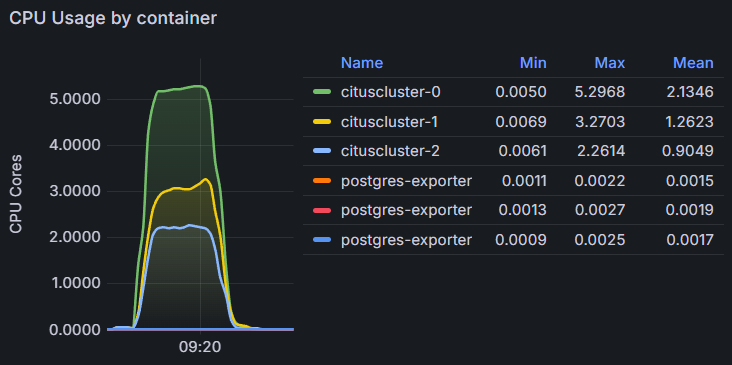
\includegraphics[width=1\textwidth]{resources/chapter-4/citusdata-usage.png}
    \caption{Penggunaan CPU CitusData (f2t3)}
    \label{fig:citusdata-usage}
\end{figure}

\textit{Node} cituscluster-0 merupakan koordinator dengan sisanya adalah \textit{worker}. Pada kasus ini, beban pada koordinator cukup tinggi hingga dua kali beban pada satu instans \textit{worker}. Berdasarkan hal tersebut, diketahui bahwa \textit{overhead} pada koordinator memiliki dampak yang signifikan pada kinerja CitusData.

Setelah ditelusuri, terdapat sebuah diskusi pada repositori CitusData yang membahas kinerja CitusData yang buruk pada \textit{benchmark} TPC-C. Terdapat sebuah komentar yang menjawab mengapa hal ini memang wajar. Selain karena CitusData membutuhkan beberapa \textit{network round-trip}, beban TPC-C lebih banyak pada \textit{query planning} dibandingkan dengan eksekusinya \parencite{Slot2020}.

Beban TPC-C dan beban penjualan tiket memiliki kemiripan, sehingga hal yang sama juga berlaku pada kasus ini. Pada penjualan tiket, beban basis data terdiri atas banyak kueri baca dan kueri tulis yang sebenarnya cukup ringan, sehingga koordinator mengalami beban yang tinggi karena harus melakukan tambahan \textit{query planning} untuk koordinasi.

Terdapat alternatif \textit{benchmark} TPC-C yang juga dibahas pada komentar tersebut, yaitu \textit{benchmark} HammerDB. HammerDB menyimpan logika pengujian pada \textit{stored procedure} PostgreSQL. Citus dapat mendelegasikan pemanggilan prosedur tersebut dengan \textit{overhead} yang jauh lebih kecil dan dengan jumlah \textit{network round-trip} yang lebih sedikit \parencite{Slot2020}. Hal ini dibahas lebih lanjut pada artikel yang membahas penggunaan \textit{distributed function} untuk latensi yang lebih baik pada CitusData versi 9 \parencite{Slot2020faster}.

Pendekatan dengan \textit{stored procedure} merupakan alternatif yang dapat dipelajari lebih lanjut pada tugas akhir lain untuk pengoptimalan yang lebih optimal. Meskipun begitu, permasalahan dari pendekatan ini adalah pemindahan logika bisnis dari kode aplikasi ke basis data. Selain karena keterbatasan sintaks dan dukungan integrasi, logika bisnis yang dijalankan pada level aplikasi belum tentu dapat diterjemahkan secara persis menjadi \textit{stored procedure} PostgreSQL.

\subsubsection{Pembahasan Kinerja YugabyteDB}

Sebagaimana ditunjukkan pada Tabel \ref{table:latensi-kueri}, latensi YugabyteDB memang dapat diprediksi karena mekanisme di baliknya yang menggunakan konsensus berbasiskan Raft. Setiap penulisan harus menunggu kluster mencapai konsensus terlebih dahulu, sehingga latensinya lebih tinggi. Meskipun begitu, latensi YugabyteDB yang lebih lambat hingga 100-200x dibandingkan dengan PostgreSQL merupakan hal yang tidak diprediksi.

Pada kasus yang lebih sederhana, seorang pengguna melaporkan penurunan kinerja hingga 300x lebih lambat dibandingkan dengan PostgreSQL. Meski setelah beberapa tahun berlalu telah banyak dilakukan pengoptimalan pada YugabyteDB, referensi hasil pengujian ini tetap dapat dianggap relevan sebagai validasi bahwa penurunan kinerja seperti ini memang juga terjadi pada kasus lain \parencite{yugabyteIssuePerformance}.

Permasalahan latensi ini dapat diterima apabila kinerja YugabyteDB juga diiringi dengan keunggulan dari aspek lain, seperti kemampuan menangani keadaan perebutan tiket dengan baik dan kestabilan kluster yang baik. Meskipun begitu, hal ini juga tidak dapat ditunjukkan oleh YugabyteDB. Gambar \ref{fig:metrics-f3t1} menunjukkan gambaran kinerja YugabyteDB saat berjalan dengan baik. Pada pengujian ini, terdapat beberapa waktu ketika YugabyteDB menangani permintaan pemesanan dengan latensi normal (sekitar 1,5 detik) yang ditunjukkan oleh garis merah. Meskipun begitu, terdapat periode ketika latensinya meningkat hingga 10 detik.

\begin{figure}[H]
    \centering
    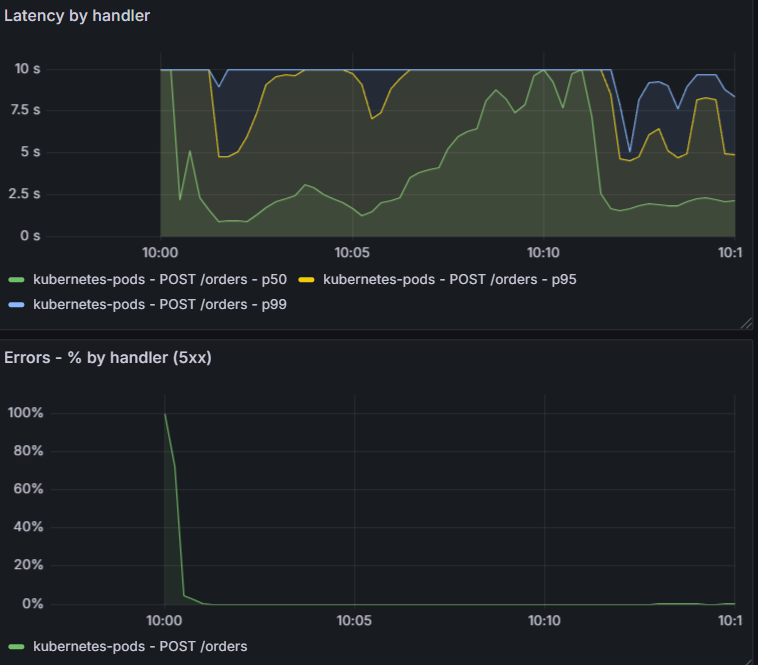
\includegraphics[width=1\textwidth]{resources/chapter-4/latensi-yugabyte-success.png}
    \caption{Metrik Pemrosesan Pesanan (f3t2)}
    \label{fig:metrics-f3t1}
\end{figure}

Hasil ini merupakan hasil paling baik yang dapat diperoleh dari pengujian YugabyteDB. \textit{Tuning} lebih lanjut seperti mengubah batas koneksi dan penambahan beban membuat YugabyteDB mengalami kegagalan penuh. Kegagalan penuh pada YugabyteDB di bawah beban yang lebih tinggi diilustrasikan pada Gambar \ref{fig:metrics-f3t2}. Grafik bawah (Errors - \% by handler) menunjukkan bahwa tingkat kesalahan untuk POST /orders secara rata-rata konsisten berada di atas 90\%, dan sering kali mencapai 100\%. Akibatnya, grafik atas (Latency by handler) menunjukkan data latensi yang tidak valid karena hampir tidak ada permintaan yang berhasil diproses. Selain itu, latensi pemrosesan pesanan secara konsisten berada di atas 10 detik.

\begin{figure}[H]
    \centering
    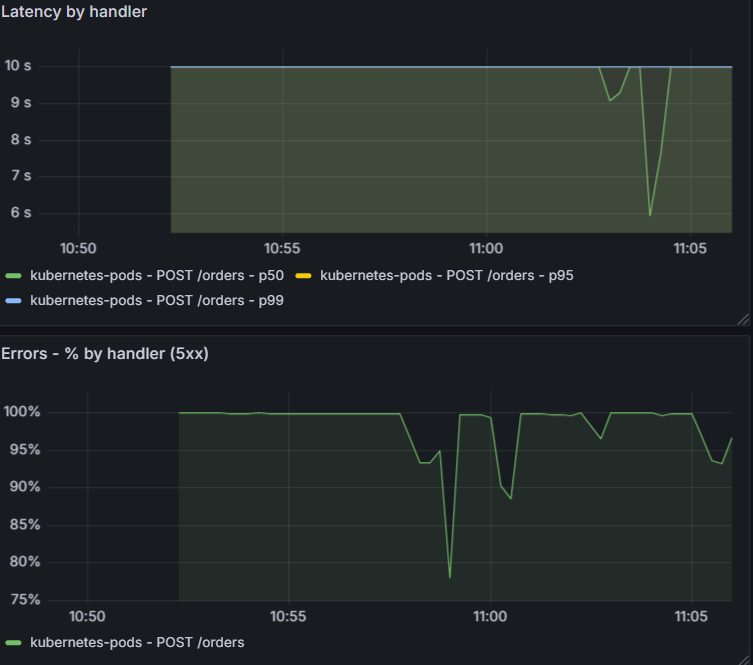
\includegraphics[width=1\textwidth]{resources/chapter-4/latensi-yugabyte-fail.png}
    \caption{Metrik Pemrosesan Pesanan (f3t2)}
    \label{fig:metrics-f3t2}
\end{figure}

Selama pengujian, terdapat beberapa kasus ketika salah satu \textit{node} YugabyteDB mati, sehingga menyebabkan kluster basis data mati dan tidak dapat menangani permintaan selama beberapa waktu. Ketidakstabilan kluster ini juga merupakan hal yang menjadi permasalahan selama pengujian.

Setelah ditelusuri, laju pemrosesan kueri saat YugabyteDB mengalami kegagalan sebagaimana ditunjukkan pada Gambar \ref{fig:metrics-f3t2} mengalami penurunan yang cukup tajam dibandingkan saat YugabyteDB berjalan cukup baik sebagaimana ditunjukkan pada Gambar \ref{fig:metrics-f3t1}. Penyebab pasti hal ini belum dapat diidentifikasi hingga pengujian selesai dilaksanakan. Akan tetapi, dapat diasumsikan bahwa setelah melewati beban tertentu, YugabyteDB mulai kesulitan menangani beban yang diberikan, sehingga kegagalan mulai sering terjadi dan laju pemrosesan kueri menjadi lebih lambat.

Gambar \ref{fig:yugabytedb-throughput} menunjukkan total kueri dan latensi pada YugabyteDB saat berjalan dengan baik. Perhatikan grafik kiri yang berwarna biru (kueri UPDATE dan INSERT). Rata-rata operasi adalah 1000 operasi per detik. Perhatikan grafik kanan. Garis berwarna biru muda dan coklat tua menunjukkan latensi operasi INSERT dan UPDATE. Rata-rata latensi operasi tersebut adalah 50 milisekon (garis merah). Garis berwarna coklat muda menunjukkan latensi operasi TRANSACTION dengan rata-rata latensi 100 milisekon (garis hijau).

\begin{figure}[H]
    \centering
    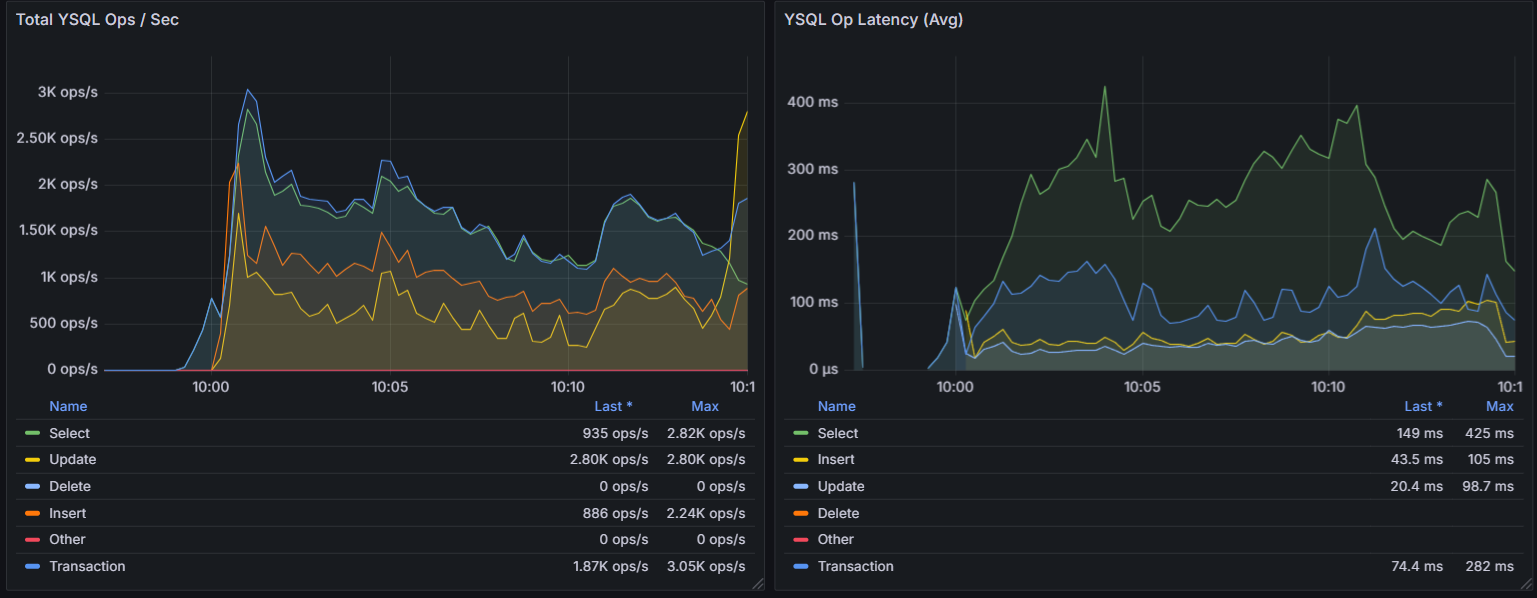
\includegraphics[width=1\textwidth]{resources/chapter-4/yugabyte-ops.png}
    \caption{\textit{Throughput} Kueri Pada YugabyteDB}
    \label{fig:yugabytedb-throughput}
\end{figure}

Masalah lain yang berhasil diidentifikasi pada YugabyteDB ini adalah masalah manajemen koneksi. Setelah beberapa kali pengujian, tidak ditemukan kombinasi pengaturan koneksi yang memberikan kinerja yang baik, baik itu jumlah koneksi dari sisi klien ke PGCat atau pun jumlah koneksi dari PGCat ke TServer. \textit{Pooler} bawaan YugabyteDB, yaitu YSQL Connection Manager juga tidak memberikan perubahan kinerja. Selain itu, pengujian tanpa \textit{pooler} (menggunakan \textit{direct connection}) juga sudah dicoba dan tetap tidak memperoleh hasil yang baik.

Singkat cerita, YugabyteDB kesulitan menangani beban koneksi yang ada pada pengujian dan memiliki masalah pada kestabilan kluster untuk dapat digunakan secara andal. Hal ini mungkin saja berubah apabila YugabyteDB diberi lebih banyak sumber daya atau lebih banyak \textit{node}.

\subsection{Pengoptimalan Kueri Baca}

\subsubsection{Kueri Ketersediaan Area}

Operasi baca ketersediaan area merupakan \textit{endpoint} yang cukup banyak dipanggil, terutama ketika ketersediaan tiket mulai menipis dan pengguna mencoba mengeksplorasi lebih banyak area. Gambar \ref{fig:throughput-get-area} menunjukkan metrik pada pengujian f5t2 dengan puncak pemanggilan sebanyak 1700 rps.

\begin{figure}[H]
    \centering
    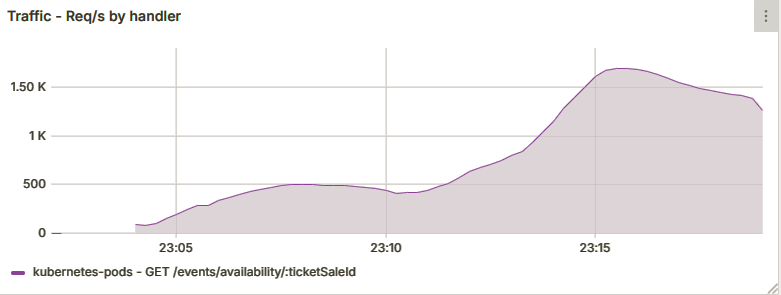
\includegraphics[width=1\textwidth]{resources/chapter-4/throughput-area-availability.png}
    \caption{Metrik \textit{Throughput} Baca Ketersediaan Area (f5t2)}
    \label{fig:throughput-get-area}
\end{figure}

Selanjutnya, Gambar \ref{fig:latency-get-area} menunjukkan latensi operasi baca. Rata-rata latensi ditunjukkan dengan garis berwarna ungu yang sangat dekat dengan garis dasar. Berdasarkan interaksi dengan grafik (tidak terlihat pada grafik), latensi rata-rata operasi ini adalah 2,5 hingga 4,5 milisekon. Hal ini menunjukkan bahwa pengoptimalan kueri ketersediaan area dengan menggunakan Redis merupakan pendekatan yang sangat efektif, terutama dalam meringankan beban pada basis data.

\begin{figure}[H]
    \centering
    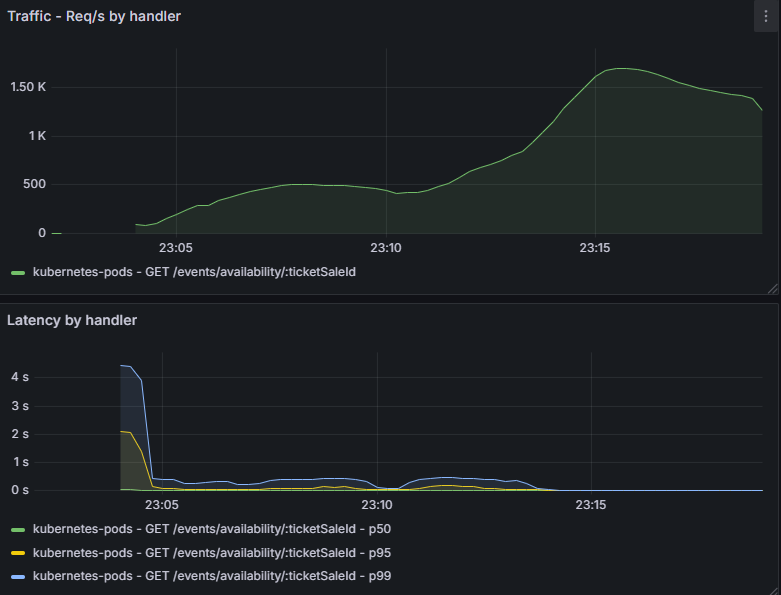
\includegraphics[width=1\textwidth]{resources/chapter-4/latency-area-availability.png}
    \caption{Metrik Latensi Baca Ketersediaan Area (f5t2)}
    \label{fig:latency-get-area}
\end{figure}

\subsubsection{Kueri Ketersediaan Kursi}

Operasi baca ketersediaan kursi tidak dipanggil sebanyak operasi sebelumnya. Pada Gambar \ref{fig:throughput-get-seat}, puncak pemanggil operasi ini adalah 350 rps. Hal ini terjadi karena tidak semua tiket merupakan tiket dengan nomor kursi dan pengguna tidak akan memanggil operasi ini apabila tidak menemukan area yang memenuhi kriterianya.

\begin{figure}[H]
    \centering
    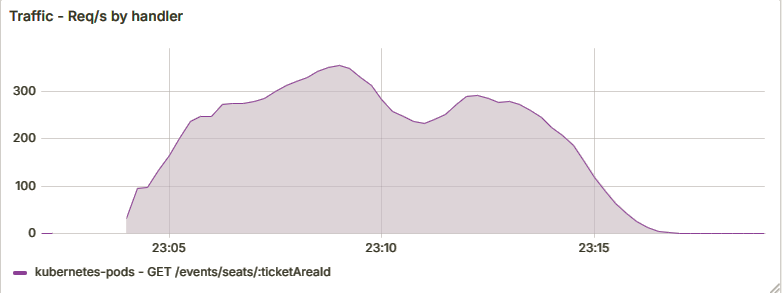
\includegraphics[width=1\textwidth]{resources/chapter-4/throughput-seat-availability.png}
    \caption{Metrik \textit{Throughput} Baca Ketersediaan Kursi (f5t2)}
    \label{fig:throughput-get-seat}
\end{figure}

Meskipun begitu, pengoptimalan kueri ini tidak berjalan dengan cukup baik sebagaimana ditunjukkan pada Gambar \ref{fig:latency-get-seat}. Rata-rata latensi (P50 dan garis berwarna ungu) memiliki nilai mulai dari 40 milisekon hingga 1.75 sekon (apabila mengesampingkan latensi di awal saat jumlah koneksi masih sedikit). Di sisi lain, latensi P95 (garis berwarna biru) cukup tinggi dengan banyak periode ketika latensinya berada di atas  2,5 detik. Hal ini menunjukkan bahwa penggunaan tembolok singkat (waktu hidup 150 milisekon) tidak begitu efektif.

\begin{figure}[H]
    \centering
    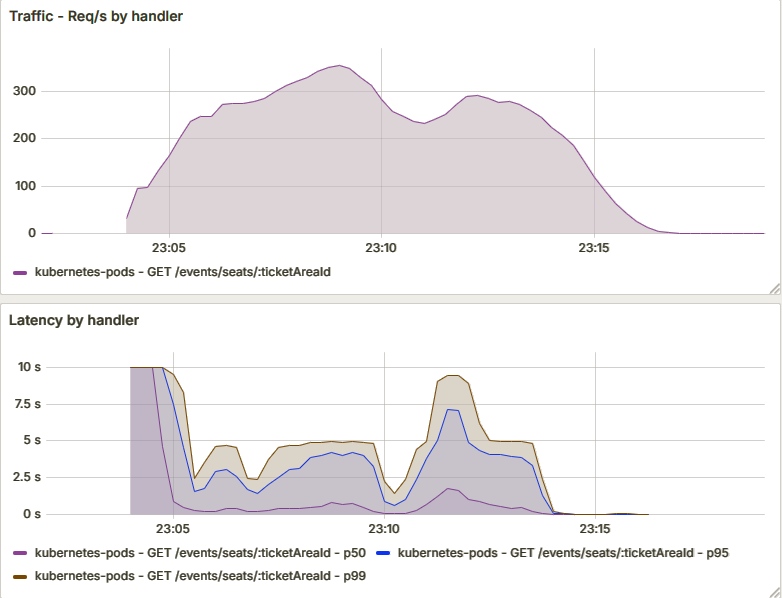
\includegraphics[width=1\textwidth]{resources/chapter-4/latency-seat-availability.png}
    \caption{Metrik Latensi Baca Ketersediaan Kursi (f5t2)}
    \label{fig:latency-get-seat}
\end{figure}

Tingginya latensi operasi ini dapat terjadi karena beberapa hal berikut:

\begin{enumerate}
    \item Tembolok yang bersifat lokal pada level aplikasi.
    \item Sebaran pengguna yang membaca ID area yang berbeda-beda.
    \item Waktu hidup yang terlalu singkat.
\end{enumerate}

Kombinasi hal tersebut membuat \textit{cache hit} operasi ini rendah sehingga tidak efektif. Rendahnya \textit{cache hit} ini ditunjukkan dengan tingginya latensi operasi ini. Meskipun begitu, tidak ada angka pasti yang menunjukkan berada \textit{cache hit} operasi ini. Selain itu, latensi ini menunjukkan bahwa operasi ini merupakan operasi yang cukup berat yang ditandai dengan latensi yang ada dan merupakan hal yang dapat menjadi fokus pengoptimalan di masa mendatang. Sebagaimana ditunjukkan pada pengoptimalan sebelumnya, pengoptimalan penggunaan Redis bisa menjadi alternatif yang dapat dieksplorasi lebih lanjut.

\subsection{Penggunaan Pengendalian Aliran}

Gambar \ref{fig:latency-nofc} menunjukkan latensi pemrosesan pesanan sistem tanpa pengendalian aliran. Perhatikan garis berwarna ungu (dan garis merah). Rata-rata latensi operasi tersebut sekitar 1,5 detik.

\begin{figure}[H]
    \centering
    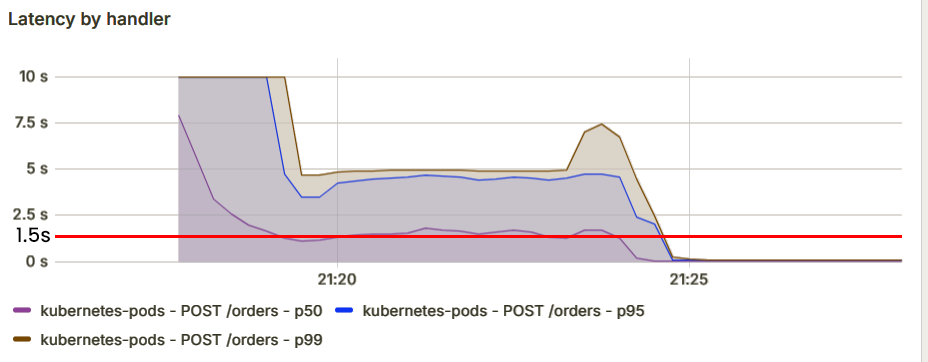
\includegraphics[width=1\textwidth]{resources/chapter-4/latency-nofc-pg-stress-0.png}
    \caption{Latensi Pemrosesan tanpa Pengendalian Aliran}
    \label{fig:latency-nofc}
\end{figure}

Selanutnya, Gambar \ref{fig:latency-fc} menunjukkan latensi pemrosesan pesanan sistem dengan pengendalian aliran. Saat berjalan baik (garis ungu landai), latensip emrosesan berada pada angka ratusan milisekon. Meskipun begitu, rata-rata latensi pemrosesan ini pada banyak waktu berada di atas 10 detik.

\begin{figure}[H]
    \centering
    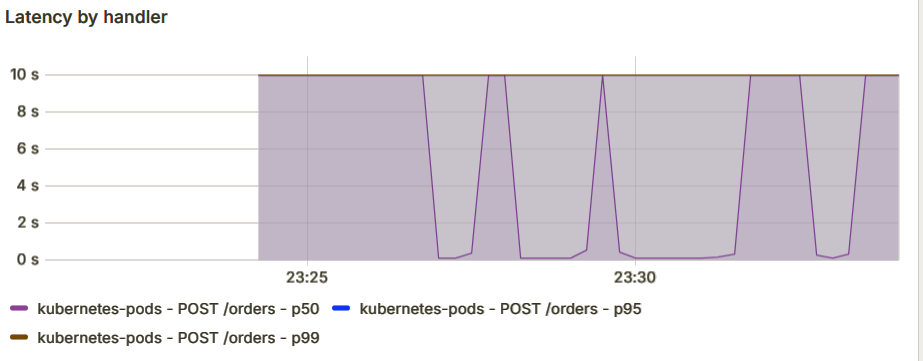
\includegraphics[width=1\textwidth]{resources/chapter-4/latency-fc-pg-stress-0.png}
    \caption{Latensi Pemrosesan dengan Pengendalian Aliran}
    \label{fig:latency-fc}
\end{figure}

Selanjutnya, perhatikan laju pemrosesan berdasarkan kode respons sebagaimana ditunjukkan pada Gambar \ref{fig:rps-fc-pg-stress-0} dan Gambar \ref{fig:rps-nofc-pg-stress-0}. Pada Gambar \ref{fig:rps-fc-pg-stress-0}, puncak laju pemrosesan adalah 550 rps (perhatikan puncak garis berwarna ungu). Pada Gambar \ref{fig:rps-nofc-pg-stress-0}, puncak laju pemrosesan adalah 570 rps (perhatikan puncak garis berwarna ungu). Meskipun memiliki latensi yang lebih tinggi, laju pemrosesan puncak varian ini sama dengan laju pemrosesan puncak pada sistem referensi. Oleh karena itu, latensi yang tinggi tidak serta merta membuat laju pemrosesan lebih lambat.

\begin{figure}[H]
    \centering
    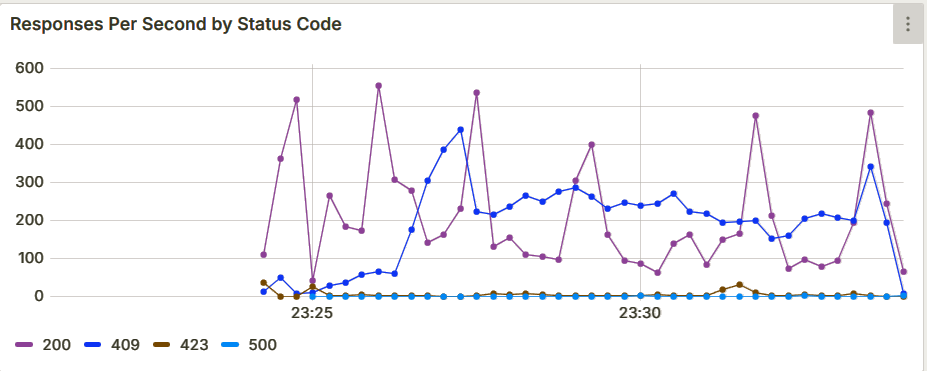
\includegraphics[width=1\textwidth]{resources/chapter-4/rps-fc-pg-stress-0.png}
    \caption{Laju Pemrosesan dengan Pengendalian Aliran}
    \label{fig:rps-fc-pg-stress-0}
\end{figure}

\begin{figure}[H]
    \centering
    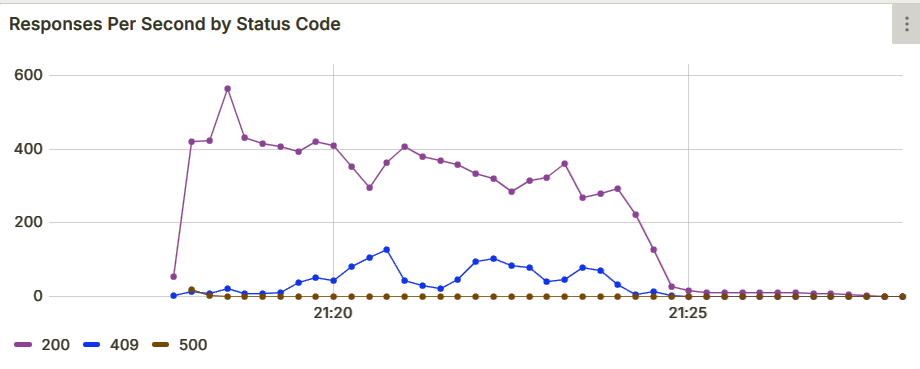
\includegraphics[width=1\textwidth]{resources/chapter-4/rps-nofc-pg-stress-0.png}
    \caption{Laju Pemrosesan tanpa Pengendalian Aliran}
    \label{fig:rps-nofc-pg-stress-0}
\end{figure}

Latensi yang tinggi pada sistem ini merupakan konsekuensi yang tidak diinginkan karena penggunaan RabbitMQ dan pemisahan pemrosesan dengan \textit{worker} (pengendalian aliran dengan sistem antrean). Dengan menggunakan antrean melalui RabbitMQ, sebuah pemesanan harus dikirimkan melalui RabbitMQ, menunggu diproses di \textit{worker}, diproses, dikirim kembali ke Ticket Server melalui RabbitMQ, dan Ticket Server menunggu hingga respons pemesanan diterima. Penambahan \textit{network round-trip} ini yang membuat lantesi menjadi sangat tinggi. Meskipun begitu, sistem tetap memproses pesanan sebagaimana mestinya.

Kode respons 409 yang tinggi pada varian pengendalian aliran juga merupakan dampak dari implementasi sistem antrean yang kurang optimal. Dengan latensi yang tinggi, terdapat lebih banyak \textit{time window} ketika sebuah kursi seharusnya sudah dipesan tetapi pemrosesan belum sepenuhnya berhasil. Oleh karena itu, kemungkinan pengguna virtual memesan tiket yang sudah dipesan menjadi lebih tinggi. Hal ini juga yang menyebabkan laju pemrosesan yang berhasil terkadang turun. Pada sistem antrean dengan latensi yang lebih rendah, kode respons 409 seharusnya menjadi lebih berkurang.

Meskipun implementasi sistem antrean kurang optimal, terdapat beberapa hal positif yang dapat dibahas. Perhatikan Tabel \ref{table:latensi-kueri-fc-nofc} yang membandingkan latensi kueri pada varian dengan pengendalian aliran (FC) dan tanpa pengendalian aliran (No FC):

\begin{table}[H]
    \centering
    \caption{Latensi Eksekusi Kueri pada Pengendalian Aliran dalam Milisekon}
    \label{table:latensi-kueri-fc-nofc}
    \begin{tabular}{|l|l|l|}
        \hline
        \textbf{Kueri}        & \textbf{No FC} & \textbf{FC} \\
        \hline
        LockFreeStandingSeats & 8.5            & 0.98        \\
        \hline
        LockNumberedSeats     & -              & -           \\
        \hline
        InsertOrder           & 0.2            & 0.2         \\
        \hline
        InsertIssuedTiket     & 0.28           & 0.3         \\
        \hline
        InsertInvoice         & 0.12           & 0.12        \\
        \hline
    \end{tabular}
\end{table}

Tidak ada perbedaan latensi pada operasi tulis (InsertOrder, InsertIssuedTiket, dan InsertInvoice). Meskipun begitu, latensi untuk \textit{lock} kursi (LockFreeStandingSeats) pada varian dengan pengendalian aliran jauh lebih kecil.

Selanjutnya, mari bandingkan latensi pemrosesan pesanan saat kode respons 409 berdasarkan Gambar \ref{fig:latency-by-code-nofc} dan Gambar \ref{fig:latency-by-code-fc}.

\begin{figure}[H]
    \centering
    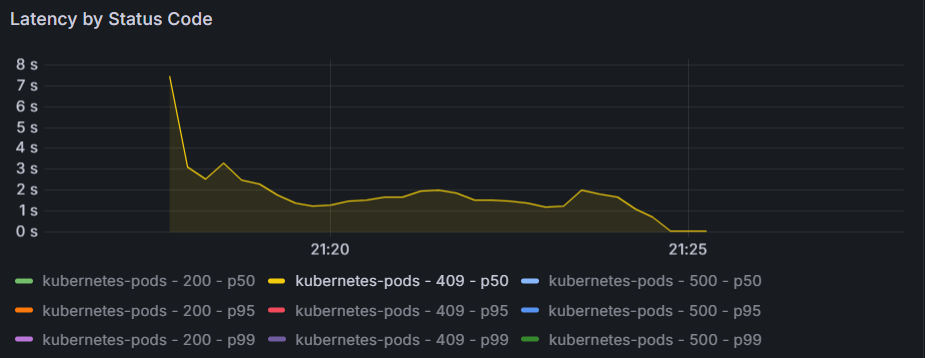
\includegraphics[width=1\textwidth]{resources/chapter-4/latency-by-code-nofc-pg-stress-0.png}
    \caption{Latensi Berdasarkan Status Kode tanpa Pengendalian Aliran}
    \label{fig:latency-by-code-nofc}
\end{figure}

\begin{figure}[H]
    \centering
    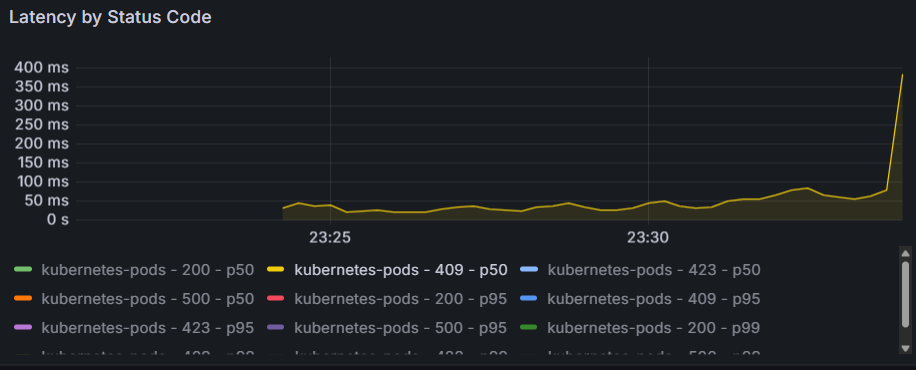
\includegraphics[width=1\textwidth]{resources/chapter-4/latency-by-code-fc-pg-stress-0.png}
    \caption{Latensi Berdasarkan Status Kode dengan Pengendalian Aliran}
    \label{fig:latency-by-code-fc}
\end{figure}

Gambar \ref{fig:latency-by-code-nofc} menunjukkan rata-rata latensi permintaan pesanan pada varian tanpa pengendalian aliran yang ditolak (kode status 409) sebesar 2 detik. Selanjutnya, Gambar \ref{fig:latency-by-code-fc} menunjukkan rata-rata latensi permintaan pada varian dengan pengenalian aliran yang ditolak (kode status 409) sebesar 50 milisekon hingga 100 milisekon (\textit{most of the time}).

Efektivitas strategi penolakan lebih awal terlihat jelas saat membandingkan latensi untuk permintaan yang ditolak (kode status 409). Perbedaan latensi ini membuktikan bahwa permintaan yang ditakdirkan gagal dapat ditolak secara signifikan lebih cepat, sebelum membebani basis data.

Hal ini menunjukkan perbedaan yang signifikan karena pesanan yang pada akhirnya akan ditolak menjadi ditolak lebih awal. Latensi tanpa \textit{early dropper} lebih tinggi karena pesanan baru akan ditolak saat sudah memasuki basis data. Selain memiliki latensi yang lebih tinggi, kasus ini juga dapat membebani basis data lebih jauh.

Secara umum, pendekatan pengendalian aliran dengan menolak pesanan lebih awal cukup baik dalam mengurangi beban basis data. Di sisi lain, pada pengujian kali ini pendekatan pengendalian aliran dengan sistem antrean tidak terlalu optimal karena latensi yang tinggi. Selain itu, beban pesanan yang masuk tidak cukup tinggi sehingga tidak cukup mengganggu keberjalanan pemrosesan pesanan. Meskipun begitu, pengendalian aliran pesanan yang masuk menunjukkan dampak positif dalam menurunkan \textit{contention} yang ditunjukkan dengan penurunan latensi salah satu kueri \textit{locking}.

Implementasi antrean yang lebih baik dan beban yang lebih tinggi seharusnya dapat menunjukkan perbedaan kinerja kedua varian lebih jauh. Agar latensi lebih baik, opsi untuk tidak menggunakan RabbitMQ juga dapat digunakan. Alih-alih memisahkan komponen Ticket Server dan Ticket Worker, antrean dapat dibuat lokal per Ticket Server. Dengan begitu, tidak perlu ada tambahan \textit{network round-trip} yang menambah latensi secara signifikan. Meskipun begitu, pendekatan ini harus memikirkan bagaimana penanganan \textit{idempotency} dan penanganan ketika pengguna mengirimkan ulang pesanan yang sama.

\subsection{Integritas Tiket Selama Perebutan Tiket}

Pengoptimalan baca dengan menggunakan Redis memungkinkan terjadinya ketidakcocokan data antara basis data dengan hasil pengoptimalan. Di sisi lain, sistem juga harus memastikan bahwa tidak ada kursi yang terjual lebih dari satu kali. Oleh karena itu, terdapat tiga hal yang diperiksa untuk memastikan integritas sistem tiket:

\begin{enumerate}
    \item Selisih agregat ketersediaan antara basis data dengan Redis pada akhirnya harus nol untuk pengoptimalan operasi baca ketersediaan area.
    \item Selisih ketersediaan antara basis data dengan Redis pada akhirnya harus nol untuk pengoptimalan pengendalian aliran bagian penolakan permintaan lebih awal (hanya berlaku pada varian pengendalian aliran).
    \item Tidak ada kursi yang terjual lebih dari satu kali.
\end{enumerate}

Gambar \ref{fig:sanity-f2t3}, Gambar \ref{fig:sanity-f3t1}, dan Gambar \ref{fig:sanity-f5t4} menunjukkan sampel hasil \textit{sanity check} selama pelaksanaan pengujian. Garis yang tidak pada angka nol menunjukkan ketidaksesuaian data.

\begin{figure}[H]
    \centering
    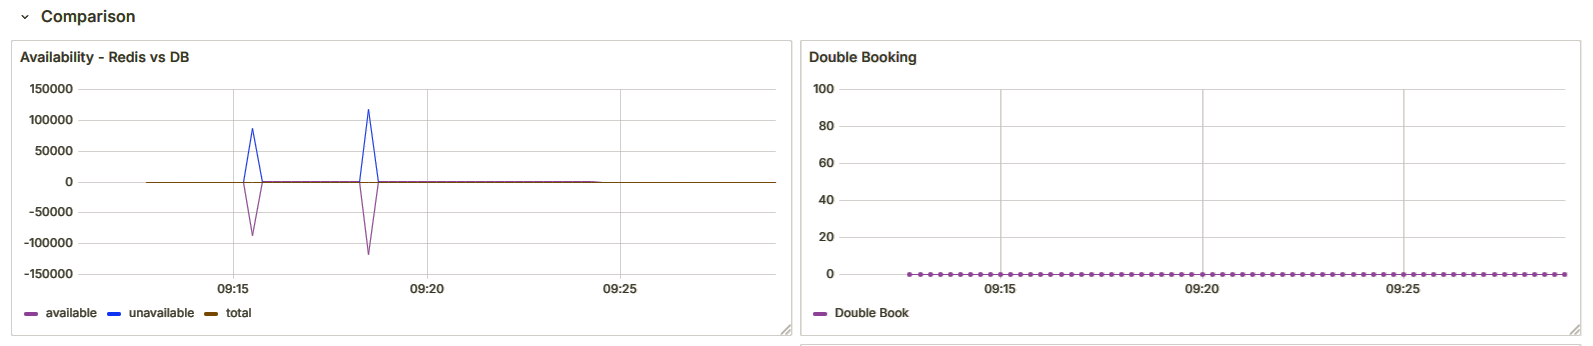
\includegraphics[width=1\textwidth]{resources/chapter-4/sanity-f2t3.png}
    \caption{Hasil \textit{Sanity Check} (f2t3)}
    \label{fig:sanity-f2t3}
\end{figure}

\begin{figure}[H]
    \centering
    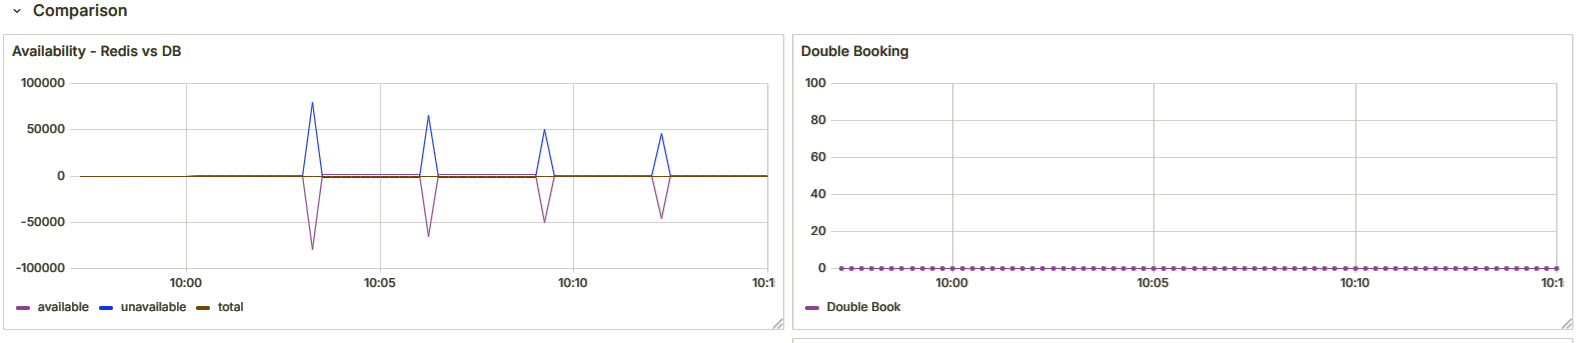
\includegraphics[width=1\textwidth]{resources/chapter-4/sanity-f3t1.png}
    \caption{Hasil \textit{Sanity Check} (f3t1)}
    \label{fig:sanity-f3t1}
\end{figure}

\begin{figure}[H]
    \centering
    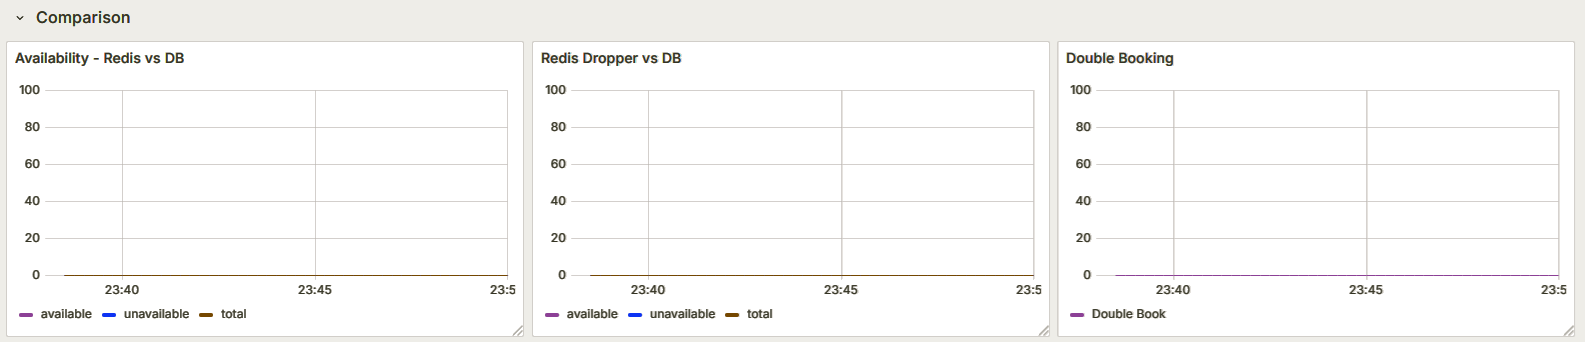
\includegraphics[width=1\textwidth]{resources/chapter-4/sanity-f5t4.png}
    \caption{Hasil \textit{Sanity Check} (f5t4)}
    \label{fig:sanity-f5t4}
\end{figure}

Berdasarkan sampel di atas, terdapat beberapa waktu terjadinya ketidaksesuaian data yang pada akhirnya konsisten (Gambar \ref{fig:sanity-f2t3} dan Gambar \ref{fig:sanity-f3t1} pada grafik kiri). Setelah ditelusuri, hal tersebut terjadi karena masalah pada pengumpulan data yang mengalami kegagalan memperoleh data yang lengkap. Hal ini didukung dengan fakta bahwa selisih nilainya memang sangat ekstrem. Mengingat sepanjang waktu setiap grafik tersebut landai dan berada pada angka nol, dapat disimpulkan bahwa tidak terjadi ketidaksesuaian data pada sistem. Oleh karena itu, dapat disimpulkan bahwa implementasi yang ada sekarang telah menjamin kesesuaian data dan berhasil menjamin bahwa tidak ada kursi yang terjual lebih dari satu kali.
